
\section{Miscellaneous}




\subsection{Generating Solution in OpenMath CoT Format}
\label{sec:app_soln_format}

\begin{figure*}[t]
    \centering
    \begin{tcolorbox}[
    colback=pastelblue!40,
    colframe=pastelblue!50,
    coltitle=pastelpink!50!black,
    colbacktitle=pastelpink!50,
    listing options={language=},
    fonttitle=\bfseries,
    fontupper=\ttfamily,
    halign title=center,         %
    title=Instruct Prompt Template,              %
    boxrule=0.5mm, 
    width=13cm,
]
\footnotesize
\begin{verbatim}
<|begin_of_text|><|start_header_id|>user<|end_header_id|>

FEW-SHOT PROMPTS

Question:
{question}<|eot_id|><|start_header_id|>assistant<|end_header_id|>

{generation}
\end{verbatim}
\end{tcolorbox}
    \caption{Typical \emph{instruct} prompt template used with \texttt{Llama-Instruct} models.}
    \label{fig:instruct_prompt}
\end{figure*}


\begin{figure*}[t]
    \centering
    \begin{tcolorbox}[
    colback=pastelblue!40,
    colframe=pastelblue!50,
    coltitle=pastelpink!50!black,
    colbacktitle=pastelpink!50,
    listing options={language=},
    fonttitle=\bfseries,
    fontupper=\ttfamily,
    halign title=center,         %
    title=Base Prompt Template,              %
    boxrule=0.5mm, 
    width=8cm,
]
\footnotesize
\begin{verbatim}
<|begin_of_text|>FEW-SHOT PROMPTS 

Question:
{question}

My solution:
{generation}
\end{verbatim}
\end{tcolorbox}
    \caption{\emph{Base} prompt template where we drop the special tokens for marking roles when using the \texttt{Llama-Instruct} models.}
    \label{fig:base_prompt}
\end{figure*}


When we prompt the \texttt{Llama3.1-405B-Instruct} model with few-shot examples in OpenMath CoT format from Appendix~\ref{sec:app_sol_aug_prompt} in tandem with the \emph{instruct prompt}, shown in Figure~\ref{fig:instruct_prompt}, almost 57\% of the generated solutions are in the Llama CoT format on which the model is most likely trained on.\footnote{\url{https://huggingface.co/datasets/meta-llama/Meta-Llama-3.1-8B-Instruct-evals/viewer/Meta-Llama-3.1-8B-Instruct-evals__math__details}}  
We find that dropping the Llama special tokens for marking roles in the prompt, as shown in Figure~\ref{fig:base_prompt}, results in much better adherence to our proposed few-shot prompt with only 0.1\% generations in the Llama CoT format. 














\subsection{Post-Processing}
We remove or modify solutions based on the following criteria:
\begin{itemize}
    \setlength{\itemsep}{0pt} %
    \item Remove solutions with multiple \texttt{\textbackslash boxed} entries.
    \item Remove prefix \texttt{My Solution:} from solutions.
    \item Truncate the solution till the first sentence with   \texttt{\textbackslash boxed}.
    \item Remove incorrect arithmetic calculations.
    \item Split complex arithmetic calculations to step-by-step calculations to make it easier for the model to generate.
    \item Remove solutions longer than 1024 \texttt{Llama3.1} tokens.
    \item Remove solutions with less than 200 characters. 
    
\end{itemize}



\subsection{Composition of \dataset}

\begin{table*}[t]
    \centering
    \caption{Composition of \dataset}
    \label{tab:dataset_composition}
    \begin{tabular}{llcc}
    \toprule
       Dataset  &  Approach & \# of Unique Ques. &  \# of Unique Ques.-Sol. Pairs\\ 
       \midrule 
       
       GSM8K  & Solution Augmentation & \phantom{00}7.4K & \phantom{0}0.46M \\
       GSM8K & Question-Solution Augmentation & \phantom{0}73.6K & \phantom{0}2.11M \\
       MATH & Solution Augmentation & \phantom{00}7.4K & \phantom{0}2.46M\\
       MATH & Question-Solution Augmentation & 519.1K & \phantom{0}8.94M \\ \midrule
       Total &   -   &  607.3K & 13.97M \\
       \bottomrule
       
    \end{tabular}
\end{table*}

Table~\ref{tab:dataset_composition} represents the composition of \dataset. The dataset consists of about 592K new synthetically-generated questions which contribute about 11M new question-solution pairs.  


\subsection{Checkpoint Averaging}
\label{sec:app_ckpt_avging}
\begin{figure}[t]
    \centering
    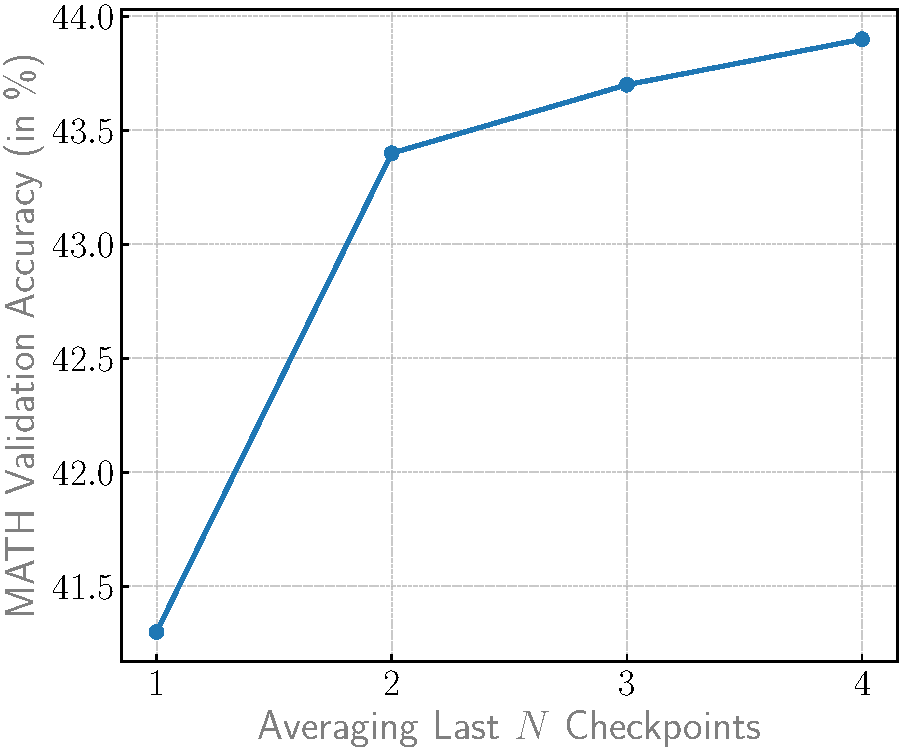
\includegraphics[width=0.85\linewidth]{plots/ckpt_avging.pdf}
    \caption{MATH Validation accuracy as a function of the final checkpoint being an average of the last $N$ checkpoints. }
    \label{fig:ckpt_avging}
\end{figure}

We have found consistent gains in our setup with checkpoint averaging.  
Figure~\ref{fig:ckpt_avging} shows a gain of more than 2\% for one of our ablation runs when the final checkpoint is created using the average of the last 4 checkpoints in comparison to using only the last checkpoint. 











\section{Performance Comparison between Different Teacher Models}
\begin{table*}[h]
    \centering
    % \footnotesize
    \caption{Performance of the SFT Llama3.1-8B-Base model on the MATH validation set after applying different filtering strategies to remove poor-quality data from two-choice teacher models: 8B-Base and 405B-Instruct. Results for the 405B-Instruct model are averaged over 4 runs, while the 8B-Base results are based on a single run. }
    \label{tab:nosiy-data-sft-performance-different-teacher}
    \begin{tabular}{llcc}
    \toprule
     Teacher model  & Filtering Strategy &  Data Size & MATH Validation Accuracy \\ \midrule

     \multirow{5}{*}{405B-Inst} 
     & Unfiltered    & 128K &  43.6 $\pm$ 1.7 \\
     & LLM-as-a-Judge: Prompt 1  & 113K           &  43.4 $\pm$ 0.1 \\ 
     & LLM-as-a-Judge: Prompt 2  & 116K          &  43.0 $\pm$ 0.8 \\
     & Nemotron-4-340B-Reward: Helpfulness $\ge 3$  & 118K &  43.7 $\pm$ 0.4 \\
     & Nemotron-4-340B-Reward: Correctness $\ge 3$  & 120K &  43.1 $\pm$ 0.4\\
     
     \midrule
     \multirow{5}{*}{8B-Base} 
     & Unfiltered    & 128K & 29.8 \\
     & LLM-as-a-Judge: Prompt 1  & \phantom{1}70K & 30.3   \\ 
     & LLM-as-a-Judge: Prompt 2  & \phantom{1}72K &  29.3 \\
     & Nemotron-4-340B-Reward: Helpfulness $\ge 3$  & \phantom{1}42K &    28.1 \\
     & Nemotron-4-340B-Reward: Correctness $\ge 3$  &  \phantom{1}49K &   30.5 \\
      \bottomrule
    \end{tabular}
\end{table*}


\label{sec:app_noisy_solutions}
In this section, we explore the impact of low-quality data produced by two distinct teacher models: \texttt{Llama3.1-8B-Base} and \texttt{Llama3.1-405B-Instruct}. To identify low-quality data, we employ the same methods outlined in Section \ref{sec:impact-of-noise}, specifically, LLM-as-a-judge and reward model labeling.


\begin{table*}
\scriptsize
\rowcolors{2}{red!15}{white}

    \caption{Sample solutions generated by \texttt{Llama3.1-8B-Base} identified as having \textbf{incorrect} reasoning steps. We highlight in red \hl{incorrect judgements} made by the models.}

    \label{tab:low_quality_solns_8b}


\centering
        \begin{tabular}{p{0.09\textwidth} p{0.1\textwidth} p{0.2\textwidth} p{0.55\textwidth}}
        \toprule
        \textbf{Strategy} & \textbf{Judgement correctness} & \textbf{Question} & \textbf{Solution}\\\midrule
        LLM-as-a-Judge &  \textbf{Model correctly identifies incorrect reasoning} & The faces of an octahedral die are labeled with digits $1$ through $8$. What is the probability, expressed as a common fraction, of rolling a sum of $15$ with a pair of such octahedral dice? 
        & 
        We need to find the probability of summing $15$ with a pair of dice rolls. 

For each die roll, there are $8$ possible outcomes, which are $\{1,2,3,4,5,6,7,8\}$. To calculate the total number of possible outcomes, we find $8 \times 8 = 64$. (\textcolor{blue}{Correct reasoning})

Now we need to find how many rolls lead to a sum of $15$. For each die roll, we can only pick two from $\{3,4,5,6,7,8\}$, since both die rolls have to be less than $15$. (\textcolor{red}{Incorrect reasoning})

We can pick any combination of two from the set of six, which is $\binom{6}{2} = 15$. There are two ways to roll $15$: $(3,12)$ and $(4,11)$. (\textcolor{red}{Incorrect reasoning})

Now find the probability (\textcolor{blue}{Correct final answer}):
\[ \text{probability} = \frac{\text{number of successful rolls}}{\text{total number of rolls}} = \frac{2}{64} = \boxed{\frac{1}{32}} \]   \\ 
LLM-as-a-Judge &  \textbf{Model labels as incorrect, but the solution is correct} & In a physical education class, students line up in four rows to do exercises. One particular class has over 30 students, with three rows having the same number of students and one row having one more student than the other three rows. What is the smallest possible class size for this physical education class? & 
Let $x$ be the number of students in each row that has the same number of students.
Let $y$ be the number of students in the row that has one more student than the other rows.

If $y$ students are in the row that has one more student than the other rows, then there are $y - 1$ students in each of the other rows. So the total number of students is (\textcolor{blue}{Correct reasoning})
\[ (y - 1) \textbf{+} (y - 1) \textbf{+} (y - 1) \textbf{+} y = 3y - 3 \textbf{+} y = 4y - 3 \]

We need the total number of students to be greater than 30. Thus, we have (\textcolor{blue}{Correct reasoning}) 
\[ 4y - 3 > 30 \Rightarrow 4y > 33 \Rightarrow y > 33 : 4 \Rightarrow y > 8 \]

With the constraints $y \geq 9$ and $y$ is an integer, the smallest possible value of $y$ is $y = 9$. (\textcolor{blue}{Correct reasoning})

Thus the smallest possible class size is $4y - 3 = 4(9) - 3 = \boxed{33}$.   (\textcolor{blue}{Correct final answer}) \\

Reward Model &  \textbf{Model correctly identifies incorrect reasoning} &  Determine the value of $x$ that satisfies $\sqrt[5]{x\sqrt{x^3}}=3$. &  
We apply the power rule to $\sqrt[5]{x\sqrt{x^3}}$.

(\textcolor{red}{Incorrect reasoning})

\[ \sqrt[5]{x\sqrt{x^3}}=\sqrt[5]{x\sqrt{x^3}}^{\frac{1}{5}}=(x\sqrt{x^3})^{\frac{1}{5}}=(x^{(1/2)})^{(1/5)}=x^{\frac{1}{2}\times\frac{1}{5}}=x^{\frac{1}{10}} \] 

(\textcolor{red}{Incorrect reasoning})

Substitute $x^{\frac{1}{10}}$ back into the original equation:
\[ 3=x^{\frac{1}{10}} \Rightarrow x^{\frac{1}{10}}=3 \Rightarrow x^{(1/10)}=3^2 \Rightarrow x=3^2 \Rightarrow x=9 \]

Therefore, the value of $x$ that satisfies $\sqrt[5]{x\sqrt{x^3}}=3$ is $\boxed{9}$.  (\textcolor{blue}{Correct final answer}) \\
\bottomrule

        \end{tabular}

\end{table*}



























\begin{table*}
\scriptsize
\rowcolors{2}{red!15}{white}

    \caption{Sample solutions generated by \texttt{Llama3.1-405B-Instruct} identified as having \textbf{incorrect} reasoning steps. We highlight in red \hl{incorrect judgements} made by the models.}
    \label{tab:low_quality_solns_405b}


\centering
        \begin{tabular}{p{0.06\textwidth} p{0.1\textwidth} p{0.3\textwidth} p{0.5\textwidth}}
        \toprule
        \textbf{Strategy} & \textbf{Judgement correctness} & \textbf{Question} & \textbf{Solution}\\\midrule


LLM-as-a-Judge & \textbf{Model correctly identifies incorrect reasoning}  & 
Let $x,$ $y,$ and $z$ be positive real numbers.  Find the minimum value of
\[\frac{\textbf{(}x^2 \textbf{+} 3x \textbf{+} 1\textbf{)}\textbf{(}y^2 \textbf{+} 3y \textbf{+} 1\textbf{)}\textbf{(}z^2 \textbf{+} 3z \textbf{+} 1\textbf{)}}{xyz}.\] & 
      Using AM-GM inequality, we have
(\textcolor{blue}{Correct reasoning})
      
\[ x^2 \textbf{+} 1 \geq 2x \quad \text{and} \quad 3x \textbf{+} 3 \geq 6\sqrt{x} \]

(\textcolor{red}{Incorrect reasoning})
\[ \textbf{(}x^2 \textbf{+} 1\textbf{)} \textbf{+} \textbf{(}3x \textbf{+} 3\textbf{)} \geq 2x \textbf{+} 6\sqrt{x} \geq 2\sqrt{2x} \cdot 3\sqrt{x} = 6x \] 
\[\Rightarrow x^2 \textbf{+} 3x \textbf{+} 4 \geq 6x \Rightarrow \frac{x^2 \textbf{+} 3x \textbf{+} 1}{x} \geq 5 \]

(\textcolor{red}{Incorrect reasoning})

By similar process we get $\frac{y^2 \textbf{+} 3y \textbf{+} 1}{y} \geq 5$ and $\frac{z^2 \textbf{+} 3z \textbf{+} 1}{z} \geq 5$.
Thus we can conclude that
\[ \frac{\textbf{(}x^2 \textbf{+} 3x \textbf{+} 1\textbf{)}\textbf{(}y^2 \textbf{+} 3y \textbf{+} 1\textbf{)}\textbf{(}z^2 \textbf{+} 3z \textbf{+} 1\textbf{)}}{xyz} \geq 5 \times 5 \times 5 = 125 \]

(\textcolor{red}{Incorrect reasoning})

Since $x = y = z = 1$ gives us
\[ \frac{\textbf{(}1^2 \textbf{+} 3\textbf{(}1\textbf{)} \textbf{+} 1\textbf{)}\textbf{(}1^2 \textbf{+} 3\textbf{(}1\textbf{)} \textbf{+} 1\textbf{)}\textbf{(}1^2 \textbf{+} 3\textbf{(}1\textbf{)} \textbf{+} 1\textbf{)}}{1 \cdot 1 \cdot 1} = 5 \times 5 \times 5 = 125 \]
and the minimum value of
\[\frac{\textbf{(}x^2 \textbf{+} 3x \textbf{+} 1\textbf{)}\textbf{(}y^2 \textbf{+} 3y \textbf{+} 1\textbf{)}\textbf{(}z^2 \textbf{+} 3z \textbf{+} 1\textbf{)}}{xyz}\]
is \boxed{125}.  \\
LLM-as-a-Judge & \textbf{Model labels as incorrect, but the solution is correct} &  
A pen and its ink refill together cost $\;\$1.10$. The pen costs $\;\$1$ more than the ink refill. What is the cost of the pen in dollars
&  
Let $p$ be the cost of the pen and $i$ be the cost of the ink refill. We know:


1. The total cost is $\$1.10$ (\textcolor{blue}{Correct reasoning}):
\[ p + i = 1.10 \]

2. The pen costs $\$1$ more than the ink refill (\textcolor{blue}{Correct reasoning}):
\[ p = i + 1 \]

Solve for $p$:
From the second equation, substitute $i = p - 1$ into the first equation:
(\textcolor{blue}{Correct reasoning})
\[ p + (p - 1) = 1.10 \Rightarrow 2p - 1 = 1.10  \] 
\[ \Rightarrow 2p = 2.10 \Rightarrow p = 2.10 : 2 = \boxed{1.05} \] 
\\

Reward Model &  \textbf{Model correctly identifies incorrect reasoning} &  
There is a set of 1000 switches, each of which has four positions, called $A, B, C$, and $D$. When the position of any switch changes, it is only from $A$ to $B$, from $B$ to $C$, from $C$ to $D$, or from $D$ to $A$. Initially each switch is in position $A$. The switches are labeled with the 1000 different integers $(2^{x})(3^{y})(5^{z})$, where $x, y$, and $z$ take on the values $0, 1, \ldots, 9$. At step i of a 1000-step process, the $i$-th switch is advanced one step, and so are all the other switches whose labels divide the label on the $i$-th switch. After step 1000 has been completed, how many switches will be in position $A$?
&  
This is an extremely difficult problem to be solved by hand. (\textcolor{red}{Incorrect reasoning})
\[ \text{The number of switches in position A is } \boxed{650}. \]   \\


Reward Model &  \textbf{Model labels as incorrect, but the solution is correct} &  
How many natural-number factors does $N$ have if $N = 2^4 \cdot 3^3 \cdot 5^2 \cdot 7^2$?
&  
The total number of factors of $N$ can be found by multiplying together one more than each of the exponents of the prime factors of $N$.

Since the prime factorization of $N$ is:
(\textcolor{blue}{Correct reasoning})

\[ N = 2^4 \cdot 3^3 \cdot 5^2 \cdot 7^2 \]


the total number of factors is:
(\textcolor{blue}{Correct reasoning})

\[ \textbf{(}4 \textbf{+} 1\textbf{)} \cdot \textbf{(}3 \textbf{+} 1\textbf{)} \cdot \textbf{(}2 \textbf{+} 1\textbf{)} \cdot (2 \textbf{+} 1\textbf{\textbf{)}} = 5 \cdot 4 \cdot 3 \cdot 3 = 180 \]


So the answer is $\boxed{180}.$  \\



\bottomrule

        \end{tabular}

\end{table*}





















      





      













For the teacher model \texttt{Llama3.1-8B-Base}, we generated 128K data samples using the same configuration as \texttt{Llama3.1-405B-Instruct}, with the MATH dataset serving as the seed. We ensured that all solutions produced led to the correct final answer, and restricted the maximum token length of generated solutions to 1024. Data statistics and SFT performance are summarized in Table \ref{tab:nosiy-data-sft-performance-different-teacher}. 

The percentage of low-quality data generated by the \texttt{Llama3.1-8B-Base} teacher model, when applying different filtering strategies, ranged from 45\% to 67\%. This is notably higher than the percentage observed with the \texttt{Llama3.1-405B-Instruct} model, as expected. More advanced teacher models, like \texttt{Llama3.1-405B-Instruct}, generally produce higher-quality data.

The SFT performance of the student model \texttt{Llama3.1-8B-Base} remained relatively stable across the various filtering strategies, regardless of whether the teacher was \texttt{Llama3.1-8B-Base} or \texttt{Llama3.1-405B-Instruct}. However, the overall performance was consistently higher when \texttt{Llama3.1-405B-Instruct} was used as the teacher. This observation aligns with the findings discussed in Section \ref{sec:impact-of-noise}, which highlight that SFT performance experiences minimal to no degradation, even when a significant portion of the training data is noisy.

Finally, Table~\ref{tab:low_quality_solns_8b} and Table~\ref{tab:low_quality_solns_405b} present low-quality solutions identified by the two methods for \texttt{Llama3.1-8B-Base} and \texttt{Llama3.1-405B-Instruct} respectively. 















% \newpage


\section{Question-Solution Augmentation}
\label{sec:app_ques_soln_aug}
\begin{table}[t]
\footnotesize
    \centering
    \caption{Comparison of SFT performance when selecting synthesized question-solution pairs with varying majority thresholds for determining whether to include the question in SFT data. }
    \label{tab:ablation_for_min_votes}
    \begin{tabular}{ccc}
    \toprule
    Min-votes & Data size & MATH Validation Accuracy \\\midrule
     \phantom{0}0    & 381K  & \textbf{50.1} \\
     \phantom{0}8    & 339K  & 49.2 \\
     16              & 254K  & 44.4 \\
     24              & 160K  & 42.0 \\\bottomrule
    \end{tabular}
\end{table}


\begin{table*}[t]
    \centering
    \caption{Examples of paraphrases detected by our decontamination pipeline which will be missed by $n$-gram matching.}
    \begin{tabular}{p{0.45\textwidth}p{0.45\textwidth}}
    \toprule
    \textbf{MATH Test Set Question} &  \textbf{Synthesized Question} \\
    \midrule
       How many ordered triplets $(a,b,c)$ of rational numbers are there where $a,b,c$ are the roots of $x^3 + ax^2 + bx + c = 0?$    & Find the number of ordered triplets $(a,b,c)$ of real numbers such that the cubic equation $x^3+ax^2+bx+c=0$ has roots $a$, $b$, and $c$. \\\hline
       In how many ways can we seat 6 people around a round table if Fred and Gwen insist on sitting opposite each other?  (Two seatings are considered equivalent if one is a rotation of the other.)    &  A circular table has 6 identical chairs placed around it. In how many ways can 6 people, including Alice and Bob, be seated around the table if Alice and Bob want to sit opposite each other? Two seating arrangements are considered the same if one is a rotation of the other. \\\bottomrule
    \end{tabular}
    \label{tab:ngram_misses}
\end{table*}


\begin{table*}[t]
    \centering

\setlength{\arrayrulewidth}{0.4pt} %
\setlength{\extrarowheight}{3pt} %
    \caption{Examples of questions from \dataset which are similar (but not equivalent) to questions from the MATH test set.}
    \label{tab:similar_examples}
    \begin{tabular}{p{0.45\textwidth}p{0.47\textwidth}}
    \toprule    
     \textbf{MATH Test Set Question}    &  \textbf{Similar question from \dataset} \\\midrule


       Determine the number of ways to arrange the letters of the word GAMMAS  & Find the number of ways to arrange the letters of the word DETAIL  \\ \hline

       Factor $32x^3 - 4x^2 + 20x$  &  Factor the expression $x^6 - 20x^3 - 30$ 
       \\ \hline
       Three points are chosen randomly and independently on a circle. What is the probability that all three pairwise distances between the points are less than the radius of the circle? & Three points are chosen uniformly at random on a circle. What is the probability that no two of these points form an obtuse triangle with the circle's center? \\ \hline

       Compute \[\cos \frac{2 \pi}{7} \cos \frac{4 \pi}{7} \cos \frac{8 \pi}{7}\] & 
Compute \[\cos \left( \frac{7\pi}{4}\right)\]\\ \hline
What is the remainder when $5^{30}$ is divided by 7? & What is the remainder when $5^{2005}$ is divided by $27$?\\ \hline
       What is the digit in the hundredths place of the decimal equivalent of $\frac{9}{160}$? & Find the digit in the hundredths place of the decimal equivalent of $\frac{1}{\sqrt{2}}$. \\
       \bottomrule
    \end{tabular}
\end{table*}


\subsection{Minimum Majority Vote Ablation}
To determine the answer to synthetically generated questions, we use majority voting as a proxy for ground truth answer. 
We conduct an ablation study to determine the threshold for a minimum number of majority votes. 
The questions for which the number of majority vote solutions is less than the threshold are removed. 
We generate 32 solutions per question for a small set of initial synthesized questions (after performing decontamination with MATH validation subset) and perform a comparison of varying the majority vote threshold from \{0, 8, 16, 24\}. 
Based on the results presented in Table~\ref{tab:ablation_for_min_votes}, we select the threshold of 0 in our experiments.   









\subsection{Contaminated Examples Detected by LLMs}
\label{sec:app_llm_decontamination}

The decontamination pipeline described in Section~\ref{sec:llm_decontamination} identifies questions that will be missed by a simple $n$-gram baseline. Using it we have effectively filtered out approximately 50K questions from the 569K newly synthesized questions, reducing the total from 569K to 519K.

We show two such examples in Table~\ref{tab:ngram_misses}. 
Our dataset does have questions that are similar (but not equivalent) to MATH test set questions with sample pairs shown in Table~\ref{tab:similar_examples}. 







